\documentclass[aspectratio=169,11pt]{beamer}
\usepackage[T1]{fontenc}
\usepackage{lmodern,booktabs,tikz}
\usetikzlibrary{positioning,arrows.meta}
\definecolor{navy}{HTML}{15324F}
\definecolor{teal}{HTML}{007F86}
\definecolor{paper}{HTML}{F3F6F9}
\setbeamercolor{normal text}{fg=navy,bg=white}
\setbeamercolor{structure}{fg=teal}
\setbeamercolor{frametitle}{fg=navy}
\setbeamercolor{block title}{fg=white,bg=navy}
\setbeamercolor{block body}{fg=navy,bg=paper}
\setbeamercolor{alerted text}{fg=teal}
\setbeamertemplate{navigation symbols}{}
\setbeamertemplate{itemize items}[circle]
\setbeamertemplate{footline}{\hfill\usebeamerfont{page number in head/foot}\color{navy}Stage 1\quad\insertframenumber/\inserttotalframenumber\hspace{5mm}\vspace{3mm}}
\setbeamersize{text margin left=9mm,text margin right=9mm}
\title{Skin-Lesion Classification}
\subtitle{Centralized baseline exploration and a minimal federated setup}
\author{Alfred Pietraru \and Stefan Dascalu}
\date{11 November 2026}

\begin{document}
\begin{frame}[plain]
  \vspace{6mm}
  {\small\color{teal}\textbf{STAGE 1 / MEDICAL IMAGE CLASSIFICATION}\par}
  \vspace{5mm}
  {\Huge\bfseries\inserttitle\par}
  \vspace{4mm}
  {\Large\insertsubtitle\par}
  \vspace{7mm}
  \textbf{Alfred Pietraru \quad Stefan Dascalu}
  \vfill
  {\small\insertdate\quad$\vert$\quad ResNet-18 $+$ ISIC 2019 $+$ Flower}
\end{frame}

\begin{frame}{What do we want to learn?}
\begin{block}{Problem}
Classify eight skin-lesion categories under severe class imbalance, then train a shared model across simulated hospitals.
\end{block}
\vspace{3mm}
\begin{enumerate}
\item How do optimization, focal loss, and resampling affect the centralized baseline?
\item Can four hospitals with non-IID data learn through FedAvg?
\item Which class and client disparities should guide Stage 2?
\end{enumerate}
\vspace{3mm}
\small This is a single-machine simulation, not a clinical evaluation or a demonstrated privacy guarantee.
\end{frame}

\begin{frame}{ISIC 2019: accuracy alone can hide weak classes}
\begin{columns}[T]
\begin{column}{0.64\textwidth}
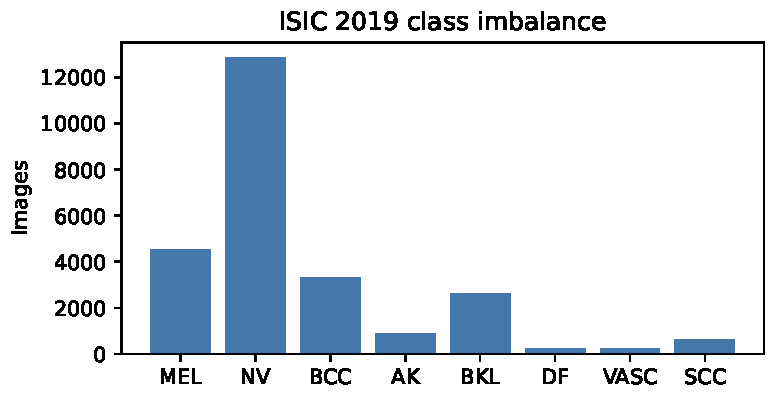
\includegraphics[width=\linewidth]{../evidence/class_distribution.pdf}
\end{column}
\begin{column}{0.33\textwidth}
\textbf{25,331 images}\\[2mm]
Eight diagnostic classes\\[4mm]
\alert{NV: 50.83\%}\\
DF: 0.94\%\\[2mm]
Largest/smallest class:\\
\textbf{53.9:1}\\[4mm]
\small Primary focus: macro-F1, supported by accuracy, class recall, and macro OvR AUC.
\end{column}
\end{columns}
\vspace{2mm}
\scriptsize Source: archived EDA class totals; historical EDA split counts are not used as experiment counts.
\end{frame}

\begin{frame}{Baseline: fine-tune the full ResNet-18}
\begin{columns}[T]
\begin{column}{0.54\textwidth}
\textbf{Training image pipeline}
\begin{enumerate}
\item Resize RGB image to $512\times512$.
\item Central $288\times288$ crop, then random $224\times224$ crop.
\item Random flips and 90-degree rotations.
\item Scale to $[0,1]$; ImageNet normalization.
\end{enumerate}
\small Validation/test: central $224\times224$ crop after resizing.\\[2mm]
\scriptsize Optimizer and transformation choices draw on Ahmad et al.~\cite{ahmad2026}, Gayatri and Aarthy~\cite{gayatri2024}, and Cino et al.~\cite{cino2025}; our pipeline adapts their ideas.
\end{column}
\begin{column}{0.43\textwidth}
\textbf{Model and split}
\begin{itemize}
\item ImageNet-initialized ResNet-18.
\item Replace classifier with eight outputs.
\item Update backbone and classifier.
\item Group by lesion ID before splitting.
\end{itemize}
\small Train / validation / test:\\
\textbf{20,236 / 2,667 / 2,428 images}\\[2mm]
Seed 42; nominal fractions 80/10/10\%.
\end{column}
\end{columns}
\vspace{3mm}
\scriptsize Missing lesion IDs fall back to image IDs; patient-level independence is not established.
\end{frame}

\begin{frame}{Reduce majority dominance, expose minority classes more often}
\centering
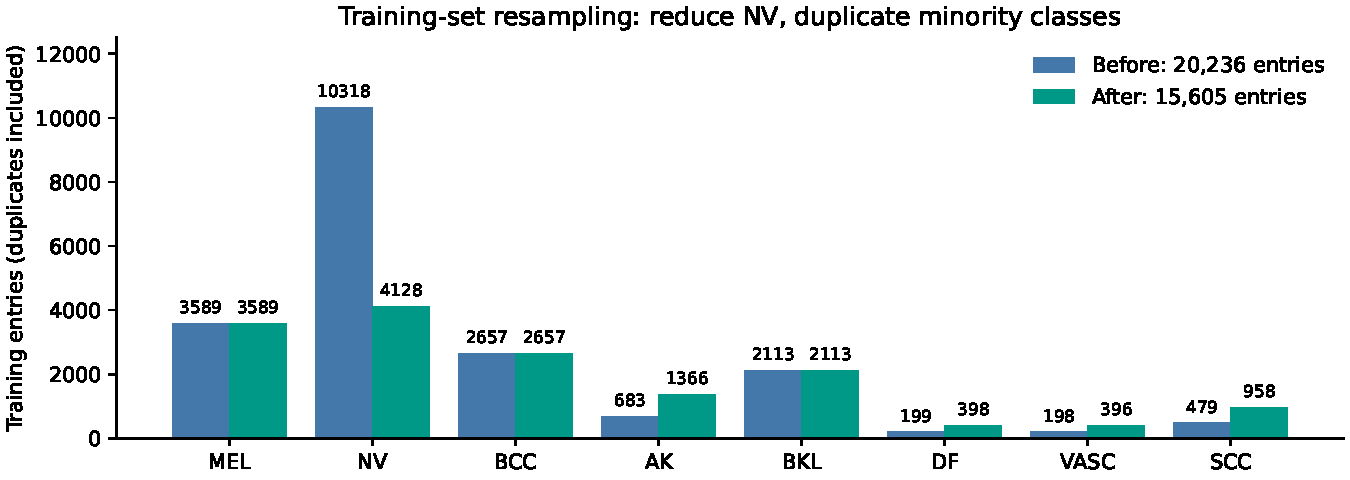
\includegraphics[width=0.92\linewidth,height=4.3cm,keepaspectratio]{../evidence/resampling_before_after.pdf}
\vspace{1mm}
\begin{itemize}
\item \textbf{Undersample NV:} remove 60\% of its training entries.
\item \textbf{Oversample AK/DF/VASC/SCC:} duplicate each entry once.
\item Largest/smallest ratio: \alert{52.1:1 $\rightarrow$ 10.4:1}; validation/test unchanged.
\end{itemize}
\scriptsize Counts from archived focal runs on the same training split. Oversampling repeats existing images; augmentation can vary their views. Rebalancing does not create new independent lesions.
\end{frame}

\begin{frame}{Centralized exploration: three completed variants}
\small
\begin{tabular}{lrrrr}
\toprule
Variant & Epochs & Test accuracy & Test macro-F1 & Test AUC\\
\midrule
AdamW + cross entropy & 12 & 0.7282 & 0.5211 & 0.9296\\
AdamW + focal loss & 18 & 0.7166 & 0.5214 & 0.9263\\
AdamW + focal + resampling & 14 & 0.6812 & 0.5017 & 0.9076\\
\bottomrule
\end{tabular}
\vspace{4mm}
\begin{itemize}
\item AdamW: learning rate $10^{-4}$; weight decay $10^{-3}$; batch size 128.
\item Focal loss: $-(1-p_t)^2\log p_t$; no class-specific alpha weights.
\item Resampling: remove 60\% of NV entries; duplicate AK/DF/VASC/SCC once.
\item Minimum-validation-loss checkpoint restored before test evaluation.
\end{itemize}
\begin{block}{Observed result}
Focal and cross-entropy test macro-F1 differ by only 0.0003. No statistical improvement is established from these single-seed runs.
\end{block}
\end{frame}

\begin{frame}{Federated setup: four hospitals, one global model}
\centering
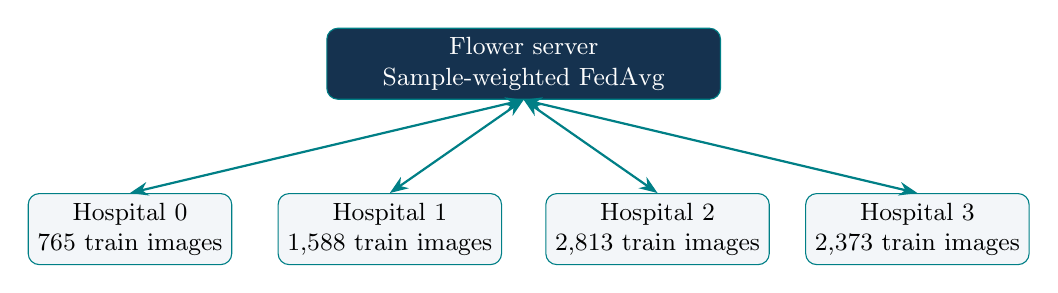
\begin{tikzpicture}[>=Stealth,box/.style={draw=teal,fill=paper,rounded corners,align=center,minimum width=2.5cm,minimum height=0.9cm},every node/.style={font=\small}]
\node[box,fill=navy,text=white,minimum width=5cm] (s) at (0,1.4) {Flower server\\Sample-weighted FedAvg};
\node[box] (a) at (-5,-0.7) {Hospital 0\\765 train images};
\node[box] (b) at (-1.7,-0.7) {Hospital 1\\1,588 train images};
\node[box] (c) at (1.7,-0.7) {Hospital 2\\2,813 train images};
\node[box] (d) at (5,-0.7) {Hospital 3\\2,373 train images};
\foreach \n in {a,b,c,d} \draw[<->,thick,teal] (s.south) -- (\n.north);
\end{tikzpicture}
\vspace{3mm}
\begin{itemize}
\item Dirichlet label skew: $\alpha=0.5$; whole lesion groups stay together.
\item 10 rounds $\times$ 5 local epochs; all four clients participate.
\item Exchange weights and metrics; validate the aggregated global model locally.
\end{itemize}
\small Optimizer state restarts each round; centralized scheduler/early stopping are not used.
\end{frame}

\begin{frame}{FedAvg learns, but validation remains much weaker}
\begin{columns}[T]
\begin{column}{0.65\textwidth}
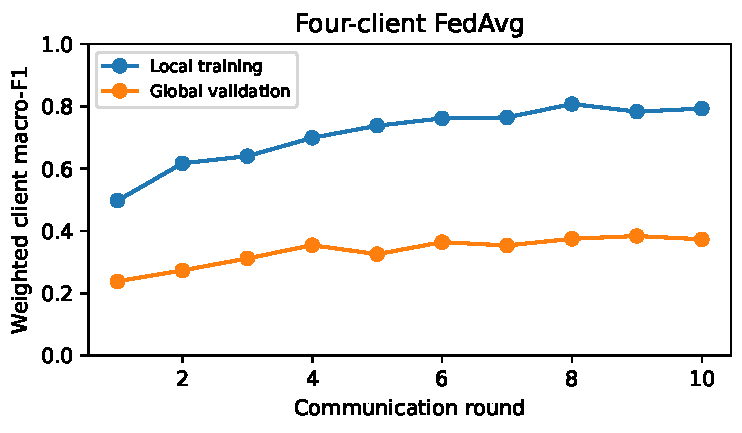
\includegraphics[width=\linewidth]{../evidence/federated_macro_f1.pdf}
\end{column}
\begin{column}{0.32\textwidth}
\textbf{Round 10 validation}\\[3mm]
Accuracy: \alert{0.6719}\\[2mm]
Weighted client\\macro-F1: \alert{0.3730}\\[5mm]
\small Highest validation macro-F1:\\
0.3837 at round 9.\\[3mm]
Saved weights: round 10.\\
No archived federated test score.
\end{column}
\end{columns}
\vspace{2mm}
\scriptsize Training scores concern local models in the last local epoch; validation scores concern the aggregated model. Macro-F1 is a sample-weighted client average, not pooled macro-F1.
\end{frame}

\begin{frame}{Centralized vs. federated: an exploratory comparison}
\small
\begin{tabular}{lrr}
\toprule
 & Centralized focal & FedAvg, round 10\\
\midrule
Target training images & 20,236 & 20,236\\
Target batch size & 128 & 128\\
Validation accuracy & 0.7338 & 0.6719\\
Validation macro-F1 & 0.5327 (pooled) & 0.3730 (weighted clients)\\
\bottomrule
\end{tabular}
\vspace{4mm}
\begin{itemize}
\item Training schedules and F1 aggregation also differ.
\item Reconstruction: focal loss and baseline preprocessing; AdamW inferred.
\end{itemize}
\begin{block}{Interpretation}
The observed gap cannot be attributed solely to federation. Next, run a matched protocol and compute pooled F1 from summed client confusion matrices.
\end{block}
\scriptsize Matched-setup target: 20,236 training images and batch size 128 for both methods. Validation scores shown are from earlier experiments, not a completed run with these matched settings.
\end{frame}

\begin{frame}{Hospital differences and Stage 2 priorities}
\begin{columns}[T]
\begin{column}{0.48\textwidth}
\textbf{Hospital-level validation, round 10}
\vspace{3mm}
\small
\setlength{\tabcolsep}{4pt}
\begin{tabular}{lrrr}
\toprule
Hospital & Images & Accuracy & Macro-F1\\
\midrule
0 & 297 & 0.4411 & 0.2651\\
1 & 538 & 0.4312 & 0.2905\\
2 & 958 & 0.8653 & 0.3846\\
3 & 874 & 0.6865 & 0.4478\\
\bottomrule
\end{tabular}
\vspace{4mm}
\small Macro-F1 ranges from \alert{0.2651 to 0.4478} across hospitals.
\end{column}
\begin{column}{0.49\textwidth}
\textbf{Stage 2 actions}
\small
\begin{enumerate}
\item \textbf{Match the evaluation protocol.}\\
Same data pool, preprocessing, initialization, validation/test sets, and explicit training budget.
\vspace{2mm}
\item \textbf{Measure who benefits.}\\
Per-class recall, worst-client scores, support counts, and uncertainty across seeds.
\vspace{2mm}
\item \textbf{Compare FedAvg with FedProx.}
\end{enumerate}
\end{column}
\end{columns}
\vspace{3mm}
\small Current evidence: a working centralized baseline and a working non-IID federated experiment.
\end{frame}

\begin{frame}{References}
\footnotesize
\begin{thebibliography}{3}
\bibitem{ahmad2026}
I. Ahmad, M. Khubaib, and S. M. Altowaijri.
Benchmarking Class Imbalance Mitigation Strategies Across Deep CNN Architectures for Skin Cancer Classification.
\emph{Diagnostics}, 16(16):2571, 2026.
\href{https://doi.org/10.3390/diagnostics16162571}{doi:10.3390/diagnostics16162571}.

\bibitem{gayatri2024}
E. Gayatri and S. L. Aarthy.
Reduction of overfitting on the highly imbalanced ISIC-2019 skin dataset using deep learning frameworks.
\emph{Journal of X-Ray Science and Technology}, 32(1):53--68, 2024.
\href{https://doi.org/10.3233/XST-230204}{doi:10.3233/XST-230204}.

\bibitem{cino2025}
L. Cino, C. Distante, A. Martella, and P. L. Mazzeo.
Skin Lesion Classification Through Test Time Augmentation and Explainable Artificial Intelligence.
\emph{Journal of Imaging}, 11(1):15, 9 January 2025.
\href{https://doi.org/10.3390/jimaging11010015}{doi:10.3390/jimaging11010015}.
PMID: 39852328; PMCID: PMC11766406.

\end{thebibliography}
\vspace{3mm}
\scriptsize These studies informed optimizer exploration, augmentation, and imbalance handling. Cino et al. also motivate future Grad-CAM analysis; test-time augmentation and explanation maps are not evaluated here.
\end{frame}
\end{document}
